\section{INTRODUCTION}
\label{S:intro}

Machine learning and control theory are two foundational but disjoint communities. Machine learning requires data to produce models, and control systems require models to provide stability and performance guarantees to plant operations. Machine learning is widely used for regression or classification, but thus far data-driven models have not been suitable for closed-loop control of physical plants. The challenge now, with using data-driven approaches, is to close the loop for real-time control and decision making.

\subsection{Motivation}
TO IMPROVE $\rightarrow$ \textcolor[rgb]{0,0,1}{Achin and Francesco}

Consider a multivariable dynamical system subject to external disturbances. The first and foremost requirement for making any decision is to obtain the underlying control-oriented predictive model of the system. With a reasonable forecast of the external disturbances, these models should predict the state of the system in the future and thus Model Predictive Control (MPC) can act preemptively to provide a desired system behavior while optimizing a desired performance. In particular, MPC has been proven to be very powerful for multivariable systems in the presence of input and output constraints, and forecast of the disturbances. The caveat is that MPC requires a reasonably accurate physical representation of the system. This makes MPC unsuitable for control of complex plants such as natural gas processing, oil refineries, boilers, manufacturing plants, and buildings where the user expertise, time, and associated sensor costs required to develop a model are very high \cite{Sturzenegger2016,vzavcekova2014}.

There are two main reasons for model complexity. 
(1) The prime contributor is the change in model properties over time. Even if the model is identified once via an expensive route, as the model changes with time, the system identification must be repeated to update the model. Thus, model adaptability or adaptive control is desirable for such systems. 
(2) A secondary reason is the model heterogeneity which further prohibits the use of model-based control. For example, unlike the automobile or the aircraft industry, each building is designed and used in a different way. Therefore, this modeling process must be repeated for every new building. 
Due to aforementioned reasons, the control strategies in such systems are often limited to fuzzy logic rules that are based on best practices. 


\paragraph{Example} \textcolor[rgb]{0.00,0.00,1.00}{As a first} example of such modeling complexity, consider the grey-box approach in \cite{Braun2002}. The scope of such approach is to predict the heat transfer rate to the air within the building. In particular, the authors addressed a single zone modeling problem using an equivalent $RC$ model. To this end, five different types of structures are considered in the example: external walls, ceiling/roof, floor, internal walls and windows. Each of these elements are represented using $3$ resistances, $2$ capacitances and $2$ temperatures, except for the windows that are represented only with resistances since they have a negligible energy storage. A model consisting of $8$ states and $9$ inputs, including disturbances such as solar radiation and others, with the instantaneous heat gain to the building air from all surfaces as output, is created for the zone. To have a complete LTI model, $9$ parameters are needed to be estimated via a non-trivial training process, using a collection of information associated with a physical description of the building (see \cite{Braun2002} for more details). Extending this result, for the building we consider in Section \ref{S:realCaseStudy} with $10$ different zones, we would need to consider a model with approximately $80$ states and $90$ parameters to be estimated.

\subsection{Modeling complexity: physics-based vs data-driven}
\textcolor[rgb]{0,0,1}{In this section we provide a more detailed example that quantifies the difference in terms of complexity when modeling a building using physical laws and data.
We compare the 2 approaches to show that the modeling technique used in our solution, i.e. data-driven modeling, eliminates several drawbacks that occur using physics-based models, such as the need to have very good knowledge of the building structure and the materials, time required to build a model, low availability of sensor measurements, etc..
\subsubsection{physics-based modeling example}
This example is taken from \cite{Sturzenegger2016}, where a building located in Allschwil, Switzerland, consisting of 6 floors, is considered. The building total conditioned floor area is of $6000\ m^2$ ca.. The building is modeled as a bilinear system constructed from physical principles. Only the second floor has been modeled, and has been assumed to represent also the others. The modeling process was divided into 4 main points:
\begin{enumerate}
	\item Building geometry and construction data were used together with first-principles laws to derive the following linear model for the building's thermal dynamics:
		\begin{equation}\label{E:RCZoneEq}
			\dot x(t) = A_x x(t) + B_q q(t).
		\end{equation}
		This model describes the behavior of zone, wall, floor and ceiling temperatures.
		Walls, floors and ceilings are considered divided into layers with different features. Therefore each zone was described with an RC network model (see Figure 3-10 in \cite{SturzeneggerTR} for more details), where the capacitances represent the states of the layers and the resistances represent the thermal resistance of the layers.
%		\begin{figure}[t]
%			\begin{center}
%				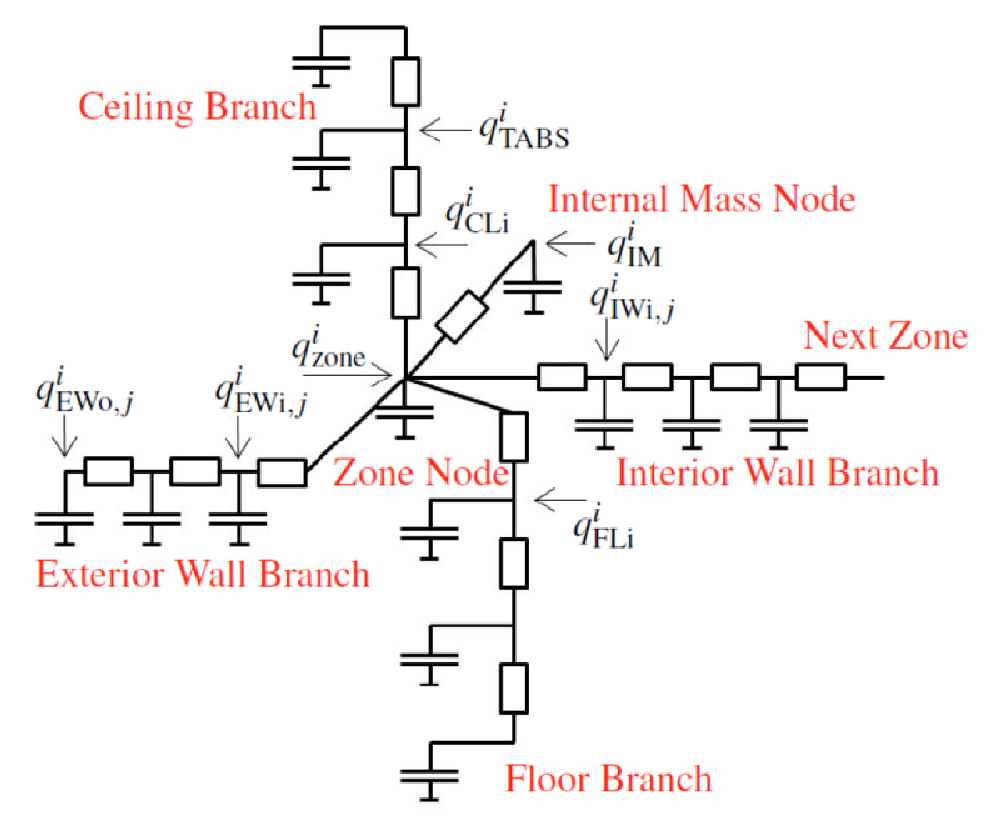
\includegraphics[width=0.6\textwidth]{figures/RC_net.eps}
%				\caption{RC model of a zone. $q$ represents the external heat fluxes}\label{F:RCnet}
%			\end{center}
%		\end{figure}
		The heat exchange between two adjacent layers, i.e. layer "a" and layer "b", was modeled to be proportional to the temperature difference of the two layers and the corresponding thermal resistance $R$, as follows
		\begin{equation}\label{E:RCHeatExchange}
			\begin{aligned}
				&C_a\dot x_a = \left(x_b(t) - x_a(t)\right)/R\\
				&C_b\dot x_b = \left(x_a(t) - x_b(t)\right)/R,
			\end{aligned}
		\end{equation}
		where $C_a$ and $C_b$ are the heat capacitances of the layers. This is done for each layer of each zone, obtaining the compact model \eqref{E:RCZoneEq}. The thermal parameters were derived from zones geometry and materials data.
	\item External heat fluxes were modeled with a bilinear model of the fluxes which are both direct into the building and indirect through elements and zones:
		\begin{equation}\label{E:RCfluxes}
			q(t) = A_q x(t) + B_{q,u}u(t) + B_{q,d}d(t) + \sum_{i=1}^{n_u}{[\left(B_{q,du,i}d(t) + D_{q,xu,i}x(t)\right)u_i(t)]},
		\end{equation}
		with $u$ the inputs and $d$ the disturbances of the system.
		Equation \eqref{E:RCfluxes} comes from a series of 20 equations analyzed in Section 3.3.1.3 of the Technical Report \cite{SturzeneggerTR}, that we do not report here for the sake of simplicity of the treatise. To model the fluxes several information have been considered in the modeling process:
	\begin{itemize}
		\item heat exchange associated with the building hull (except for windows) was modeled considering a conductive and a radiative part;
		\item  heat flux to each Thermally Activated Building System (TABS, i.e. pipes buried in the concrete slabs of the floors carrying hot/cold water) layer was modeled as a fraction of the total supplied TABS heating and cooling heat fluxes;
		\item heat flux through the windows was considered in three different parts: a radiation that directly acts with the elements in contact with the zone's air; a heat flux due to the conduction through the window; a heat flux due to the absorption of the solar radiation from the window;
		\item internal gains due to occupants, appliances and lighting were modeled as a convecting heat acting in each zone;
		\item effects due to the AHU were considered.
	\end{itemize}
	\item The system was discretized.
	\item The resulting model had approximately 300 states for the only second floor, i.e. temperature of the zones, walls and floors. The output of the system were the zone temperatures.
	Since the performance of the state estimation, that is needed to compute the optimal control inputs using MPC, heavily depends on the number of states, an approximated model with fewer states was needed.
	To this aim, different averaged temperatures of the building facades and the zones was considered, obtaining an approximated model with 35 states. The obtained approximated model was then "suitable for use in MPC" (Section 3.3.1.4 of the Technical Report \cite{SturzeneggerTR}). In particular, after the approximation, the resulting model had the following states, inputs and disturbance variables:
	\begin{itemize}
		\item 5 outputs: averaged room temperature for each group of zones (North, South, West, East, Center). The rooms are equipped with temperature sensors.
		\item 18 inputs: TABS heating heat flux; TABS cooling heat flux; averaged transmitted solar heat flux for each group of zones (North, South, West, East), that was estimated using blinds position measurements; air massflow through the energy recovering mode; air massflow bypassing the energy recovering mode; air massflow through the air cooler; AHU heat coil heat flux; lighting power for the offices for each group of zones (North, South, West, East); radiator heat flux in the corner offices (North, South, West, East).
		\item 7 disturbances: internal gains in the offices and internal gains in non-office zones, which were predicted using standard schedule; ambient temperature and solar radiation on facade (North, South, West, East), whose values were obtained through Kalman filtering, using measurements from the weather station placed on the roof of the building. This filtering is needed to take into account the shadowing of the neighboring buildings.
	\end{itemize}
\end{enumerate}
An EnergyPlus model was built for this system, and model parameters of matrices $A_x$, $B_q$, $A_q$, $B_{q,u}$, $B_{q,d}$, $B_{q,du,i}$, $D_{q,xu,i}$ were derived using geometry and materials data from such EnergyPlus model.
This was a choice of the authors, although in a previous work they used real geometry and materials data from the building. 24 parameters needed to be estimated/taken form a datasheet/computed for the considered zone model.
Although some of the parameters are in common between different zones, the others had to be found independently for each zone.
To derive the EnergyPlus model using the available measurements and to use the same control implemented in the building, the EnergyPlus model was coupled with MATLAB using BCVTB software (see \cite{SturzeneggerTR} for more details). To identify the model a total of 294 MATLAB signals were sent to the EnergyPlus model and a total of 1081 EnergyPlus signals were sent back to Matlab.}

\textcolor[rgb]{0,0,1}{This approach suffers of several drawbacks:
\begin{itemize}
	\item in order to keep the model simple, the heat exchange between layers is modeled with a linear behavior as in \eqref{E:RCHeatExchange}. Hence all the nonlinearities are neglected;
	\item in particular cases, as for example the ventilation energy, a linear model is not good enough to provide a good approximation: for this reason a bilinear model was considered.
	However, also in this case, more complex nonlinearities have been neglected due to the already high complexity of the model.
	For example, in \cite{Sturzenegger2016}, the author says "ideally one would want to formulate the optimization problem in terms of set points and operating modes that can be communicated directly to the BAS.
	However, by limiting the model to a bilinear form, this was not possible";
	\item due to the high modeling complexity, different geometries and different materials of the floors have been neglected supposing they are the same for each floor, although this is almost never true in real cases;  
	\item the resulting model was too complex, so it was further approximated to be "suitable for use in MPC" \cite{SturzeneggerTR};
	\item differently from the building geometry, that could be rebuilt by hand, materials data of the building can be unavailable for different reasons (not provided, lost, changed in time).
	Therefore they need to be estimated, hence further increasing the modeling complexity;
	\item due to the high number of states and variables involved in the modeling framework, a lot of measurements are needed to use the model to predict system's behavior.
	This can be cost expensive due to the amount of sensors needed.
	Furthermore, when some measurements are not directly available from the sensors, observers are needed to provide variables estimations.
	However, observability problems could limit the construction of the observers \cite{Dorf2011MCS}. 
\end{itemize}
}

\subsubsection{data-driven modeling example}
\textcolor[rgb]{0,0,1}{Data-driven modeling helps eliminating all the aforementioned problems...}
TO BE DONE $\rightarrow$ \textcolor[rgb]{0,0,1}{Achin}
\begin{itemize}
	\item show procedure
	\item quantify complexity
\end{itemize}


\textcolor[rgb]{0,0,1}{\textbf{Important to add this remark wrt the last bullet point (to answer the reviewer) saying that:} while in the previous case we need to measure all the variables because they are needed to compute model evolution using equations, using machine learning we don't need all the variables (so if we cannot measure everything it is not a problem). This is because the machine learning algorithm creates his internal relation between variables, so also if a variable is missing, the information of the missing variable is present in the behavior of another one. For example: if you don't have the measurement of the energy produced by a photovoltaic panel, the information of the weather conditions will take care of it.}

\textcolor[rgb]{0,0,1}{\textbf{Say also that:} since we don't need to model the state of the walls and floor layers, we don't have that many states as they are, so we don't need to approximate our model and we can consider the temperature of each room as output, without the need of considering an averaged temperature}

\textcolor[rgb]{0,0,1}{\textbf{Advantages:}
\begin{itemize}
	\item we don't need to consider averaged temperatures
	\item we don't need to filter weather data since all the noises are took into account by the machine learning algorithms
	\item we don't need to estimate any parameter
\end{itemize}}

\paragraph{physics-based vs data-driven modeling example}
TO BE DONE $\rightarrow$ \textcolor[rgb]{0,0,1}{Achin}
\begin{itemize}
	\item compare results
\end{itemize}

\paragraph{Objective} The question now is, can we employ data-driven techniques to reduce the cost of modeling and still exploit the benefits that MPC has to offer? Can we build automatic and data-driven approaches for control purposes that are also adaptive, scalable and interpretable? In this paper we address this problem introducing \textit{Data Predictive Control (DPC)} to bridge the gap between Machine Learning and Predictive Control.
\textcolor[rgb]{0,0,1}{
\subsection{Related work}
This section is divided in 3 parts:
\begin{enumerate}
	\item In Section \ref{SSS:ModelBasedWork} we provide a literature review of the approaches that make use of model-based techniques for energy optimization.
	\item In Section \ref{SSS:DataDrivenWork} we report the main works that use of data-driven methodologies for energy optimization and point out the difference with respect to our contribution.
	\item In Section \ref{SSS:PreviousWork} we underline the differences between the results presented in this work and the ones of our previous papers.
\end{enumerate}
\subsubsection{Model-based related work}\label{SSS:ModelBasedWork}
\subsubsection{Data-driven related work}\label{SSS:DataDrivenWork}}
In the literature, several studies deal with the data-driven control techniques using machine learning algorithms \cite{Hou2013}. For example, Artificial Neural Networks are exploited to create data-driven models to be used as plant simulator in closed-loop with a Supervisory Model Predictive Control in \cite{Afram2017}. In \cite{Macarulla2017} the authors proposed a predictive control strategy based on Neural Networks, for boilers control in buildings, to decide the optimal time to switch-on the plan to guarantee energy saving and thermal comfort. However, the strategy is not easily scalable to different types of plants and does not use optimization theory in the closed-loop scheme. In \cite{Costanzo2016} a reinforcement learning control strategy, called Model-Assisted Batch Reinforcement Learning, is considered to provide data-driven control for the demand response problem in HVAC systems. Reinforcement Learning is a model-free methodology and for this reason it can not be used for on-line optimization in a closed-loop predictive control scheme. In \cite{Ferreira2012} the authors considered a data-driven predictive control based on Neural Networks to guarantee energy saving and  thermal comfort in public buildings. Neural Networks are used in the closed-loop control scheme to determine a thermal comfort index based on parameters that can be measured or estimated, but no  system dynamics with internal state are included into the optimization problem. More papers related to this topic can be found in the literature, but to the best of the authors' knowledge none of them address the problem of including data-driven state models in the optimal predictive control loop, and hence allow to set up a MPC-like optimal control problem, as we do in DPC.

\textcolor[rgb]{0,0,1}{
\subsubsection{Previous work}\label{SSS:PreviousWork}
In the following, the differences with respect to our previous papers are illustrated.
\begin{itemize}
	\item In \cite{Behl2016} we	proposed an MPC-like control problem considering regression trees and ensemble methods algorithms for the Demand-Response problem. However, the proposed models allowed to optimally control the system considering only one-step lookahead prediction.
	Hence, it was not possible to use such approach to control the system considering a prediction over an horizon of arbitrary length.
	\item This problem was addressed in \cite{Jain2016}, where the regression trees algorithm was modified to allow the tree to provide multiple-output.
	Each output of the tree was then setup to provide the prediction of the system's behavior over different steps of the predictive horizon.
	This allowed us to setup an MPC-like control problem considering an arbitrary horizon.
	However, in this paper only single regression trees were considered, while ensemble methods were not took into account.
	Modeling accuracy using single trees is strongly subject to the problems of data overfitting and high variance.
	Such approach has the advantage to be extremely simple from the complexity point of view, but its application range is limited to specific kind of systems.
	\item In this work, we extend preliminary results gave in the conference paper \cite{JainCDC2017}.
	An alternative approach is proposed to improve the system's identification accuracy and robustness of the previous approach.
	More precisely, instead of considering a single tree with multiple output, we consider multiple trees with single output.
	Each tree is used to provide the prediction of the system's behavior over different steps of the horizon. With a small increase in complexity, we setup an MPC-like control problem with arbitrary horizon, that provides better results with respect to our previous work. In this paper we further extend this approach to one of the ensemble methods: the random forests.
\end{itemize}
}

\subsection{Main contribution and paper organization}
TO CLARIFY $\rightarrow$ \textcolor[rgb]{0,0,1}{Achin and Francesco}
\begin{itemize}
	\item Add more details
	\item Emphasize difference between Section 4 and Section 5
	\item Cite appendix
\end{itemize}
TO ADD $\rightarrow$ \textcolor[rgb]{1,0,0}{Tullio}
\begin{itemize}
	\item Add references for weather forecast accuracy
	\item Quantify accuracy for short-term prediction for weather forcast to justify the assumption of perfect knowledge for the disturbance
\end{itemize}
TO ADD $\rightarrow$ \textcolor[rgb]{0,0,1}{Achin and Francesco}
\begin{itemize}
	\item Add subsection in Section 5 with simulation of DPC considering disturbance with added noise and show that we still have good performance
\end{itemize}
%In our previous work \cite{Behl2016,Jain2016,JainACC2017,JainCDC2017}, we introduced the concept of DPC for receding horizon control. In this paper, we extend these results providing the following contributions.
%\begin{enumerate}
%	\item In Section \ref{S:dpc}, we formally present the two following control techniques:
%	\begin{enumerate}
%		\item DPC with regression trees, and
%		\item DPC with random forests.
%	\end{enumerate}
%	\item In Section \ref{S:proof}, we demonstrate the strength of DPC for receding horizon control via one-to-one comparison against a benchmark MPC controller using a bilinear building model whose parameters were identified using experiments on a building in Switzerland. We show that DPC captures 70\% variance in MPC and offers a comparable performance.
%	\item Section \ref{S:casestudy} describes a practical application of DPC for Demand Response, where we apply DPC to a 6 story 22 zone building model in EnergyPlus \cite{Crawley2001} for which model-based control is not economical and practical due to extreme complexity. We show scalability and efficiency of DPC in providing financial incentives to the end-customers bypassing the need for high fidelity models. We observe that DPC provides the desired power reduction with an average error of 3\%.
%	\item In Section \ref{S:realCaseStudy}, we implement DPC on the real data from an off-grid house located in L'Aquila (Italy), to find the optimal ON/OFF scheduling for the heating system in order to save energy while guaranteeing thermal comfort for the occupants. We quantify the total amount of energy saved, with respect to the classical bang-bang controller widely used in houses for temperature control, using an EnergyPlus model built specifically for the house. We show we can perform an energy saving that goes from $25.4\%$, if we guarantee thermal comfort, to $49.2\%$, if we allow very little discomfort in terms of rooms' temperature.
%\end{enumerate}